\documentclass{article}
%=============================================================================80
%	                          Packages                                     %
%==============================================================================%
% Packages
\usepackage[utf8]{inputenc}
\usepackage{graphicx}
\usepackage{amsmath}
\usepackage{amssymb}
\usepackage{braket}
\usepackage{float}
\usepackage{subcaption}
\usepackage[margin=0.7in]{geometry}
\usepackage[version=4]{mhchem}
%==============================================================================%
%                           User-Defined Commands                              %
%==============================================================================%
% User-Defined Commands
\newcommand{\be}{\begin{equation}}
\newcommand{\ee}{\end{equation}}
\newcommand{\benum}{\begin{enumerate}}
\newcommand{\eenum}{\end{enumerate}}
\newcommand{\pd}{\partial}
\newcommand{\dg}{\dagger}
%==============================================================================%
%                             Title Information                                %
%==============================================================================%
\title{Chem237: Lecture 1}
\date{4/3/18}
\author{Alan Robledo, Shane Flynn}
%==============================================================================%
\begin{document}

\maketitle

\section*{Course Overview}
The course will not directly follow the textbook, the book will be a guideline for important topics.
The lecture and homework are the most important aspects of the course.
Homework will contain both analytical and numerical problems.
Any programming language is fine for the numerical problems, however, Mathematica and other highly developed languages are discouraged.
For the numerical problems, if you are asked to make an algorithm, you CANNOT use pre-built algorithms available to the languages.

\section*{Chapter 1: Differential Equations}
A \textbf{Differential Equation} refers to an equation containing both a function and its derivatives.
An \textbf{Ordinary Differential Equation} (ODE) refers to any differential equation with functions that depend on only one independent variable.
\be
\frac{dy(x)}{dx} + y(x) = 0
\ee
In contrast a \textbf{Partial Differential Equation} (PDE) contains functions that depend on more than one independent variable.
\be
a \frac{\pd U(x,y)}{\pd x} + b \frac{\pd U(x,y)}{\pd y} = c
\ee

We can further categorize differential equations (both ODE and PDE) into linear or nonlinear (depending on the highest degree of the variable of interest).
As you can imagine, linear equations are simpler to solve compared to nonlinear and an ODE is easier to solve than a PDE.

\subsection*{Linear Equations}
Linear Equations are a general topic (not only linear differential equations); there are linear differential equations, linear algebraic equations, and etc.
Any linear equation has the form
\be
\hat{A} f(x,y,\hdots) = B(x,y,\hdots)
\ee
Where the RHS (B) is some known function, and the function f is some unknown function.
To be a linear equation, the operator $\hat{A}$ must be a \textbf{Linear Operator}.
For example, take the equation above and let $\hat{A}$ be the differential operator wrt. a single dimension.
This would then describe a linear Ordinary Differential Equation.

If the RHS of this expression (B) is equal to 0, the linear equation is called \textbf{Homogeneous} and if the RHS is anything other than 0, the linear equation is called \textbf{Inhomogeneous}.
Another way to explain this; if every term in the differential equation contains the function f or any of its derivatives, it is called Homogenous.
For example equation \ref{eq:homo_ex} is a homogenous equation.
\be \label{eq:homo_ex}
\frac{d^2y}{dx^2} + d\frac{dy}{dx} + y = 0
\ee
If there is at least one term that does not contain the function (f) and/or its derivative, it is called Inhomogeneous.
\be \label{eq:inhomo_ex}
\frac{d^2y}{dx^2} + d\frac{dy}{dx} + x = 0
\ee
Equation \ref{eq:inhomo_ex} is an inhomogenous differential equation (the x term has no dependence on y).

\subsubsection*{Homogeneous Linear Equations}
Consider equation \ref{eq:lin_homo} below
\be \label{eq:lin_homo}
\hat{A}f = 0
\ee
If we assume f$_1$ and f$_2$ are solutions to equation \ref{eq:lin_homo}, then, by the \textbf{Principle of Superposition}, we immediately know another solution; the linear combination of f$_1$ and f$_2$
\be
f_3 = c_1f_1 + c_2f_2 .
\ee
This result is true for any set of linear homogeneous ODEs: A linear combination of two unique solutions to a linear homogeneous equation gives another unique solution.

This implies that f$_1$ and f$_2$ are linearly independent functions, meaning there cannot exist a constant c such that $f_1 = cf_2$.
Checking if f$_1$ and f$_2$ are two linearly independent solutions can be done by determining the Wronskian of the two functions (if you are unfamiliar with this method feel free to ignore it).

\subsubsection*{Inhomogeneous Linear Equations}
Consider now an Inhomogeneous linear equation; equation \ref{eq:lin_inhomo}
\be \label{eq:lin_inhomo}
\hat{A}f = B
\ee
We can construct the general solution to this equation as
\be
f = f_0 + \sum_i c_i f_i
\ee
Where the $f_0$ term is known as a \textbf{Particular Solution} and the $f_i$ solutions refer to the solution of the associated homogeneous equation.
There is no formula for finding the particular solution, there are a number of methods we will explore, such as the Method of Undetermined Coefficients, and the Variation of Parameters method.

\subsection*{ODE: Linear, Homogeneous, Constant Coefficients}
We will start with the simplest class of ODEs, the linear, homogeneous, constant coefficient ODEs.
Various books use different notation for presenting ODEs.
For example, it is very common in physics to consider functions that only depend on time, x = x(t).
We may switch between using t and x as independent variables in class, since these are ordinary differential equations there will only be one variable of interest in the problem.

We will be writing lots of derivatives, some common notation for a derivative are:
\be
x^{(n)} \equiv \frac{d^n}{dt^n}x \equiv D^n x
\ee
Hopefully it is clear that D is the linear differential operator.
If you apply a linear operator n times it is still linear, therefore D$^n$ is also a linear operator.

The general form for these differential equations is
\be \label{eq:lin_cc}
\sum_{n=0}^N a_nx^{(n)} = f(t)
\ee
If we consider the homogeneous, linear, constant coefficients case, then equation \ref{eq:lin_cc} simplifies to
\be \label{eq:lin_cc_homo}
\sum_{n=0}^N a_nx^{(n)} = 0
\ee
To solve these equations, we assume a solution of the form: x(t) = e$^{\lambda t}$ and substitute this into equation \ref{eq:lin_cc_homo}.
\be
\begin{split}
    \sum_{n=0}^N a_nx^{(n)} &= 0\\
    \sum_{n=0}^N a_n \left(e^{\lambda t}\right) ^{(n)} &= 0\\
    \sum_{n=0}^N a_n \lambda^n e^{\lambda t} &= 0\\
    e^{\lambda t} \sum_{n=0}^N a_n \lambda^n &= 0\\
    \sum_{n=0}^N a_n \lambda^n &= 0\\
\end{split}
\ee

The last line is known as the \textbf{Characteristic Polynomial} and it helps us find the general solution to the linear constant coefficient ODE.
The above polynomial is of degree N, and the \textbf{fundamental Theorem of Algebra} claims that every N degree polynomial has N (potentially complex) roots that may or may not be degenerate.

The reason for using this approach (guessing an expotential) comes from mathematical intuition.
Our Differential Equation (equation \ref{eq:lin_cc_homo}) requires a function x(t) such that the function and its derivatives cancel out to satisfy the RHS.
A simple elementary function that satisfies this condition is x(t) = e$^{\lambda t}$.
To account for different multiples of the function, we include the $\lambda$ in our assumed solution, since its derivative is equal to $\lambda$ e$^{\lambda t}$.
You can probably guess that some trigonometric functions and their derivatives may also satisfy this condition.
While this may sometimes be true, it is not true generally, the expotential turns out to be a better guess.
Even if you consider a combination of sine and cosine, such a function would not always work.
Consider the example ODE below,
\be \label{eq:ode_guess}
\frac{dy}{dt} + y = 0 .
\ee
Suppose that we assume the solution to be x(t) = sin($\lambda$t) + cos($\lambda$t).
Plugging this assumed solution into the original equation (equation \ref{eq:ode_guess}) gives
\be
\lambda \cos(\lambda t) - \lambda \sin(\lambda t) + \sin(\lambda t) + \cos(\lambda t) = 0 .
\ee
There are no values of $\lambda$ that could satisfy this equation, and the guess is therefore incorrect.

We can now begin exploring the effects of both non-degenerate and degenerate roots to the characteristic polynomial.
Consider first the non-degenerate case (i.e. $\lambda_i \neq \lambda_j$).
Since each root of the polynomial gives us the $\lambda_n$ in the general solution, we can write the general solution to the ODE as
\be
x(t) = \sum_{n=1}^N c_n e^{\lambda_n t}
\ee

Finding the general solution for the degenerate case is not as straightforward.
If we have two roots that are the same (e.g. $\lambda_1$ = $\lambda_2$), we cannot form 2 unique solutions from these roots.
We would only be able to form one unique solution (each root produces the same solution).
However, there are multiple ways to show that for each repeated root, a unique solution will be given by a different multiple of the expotential.

For example, if we had a 3rd order linear ODE with repeated roots, $\lambda_1$ = $\lambda_2$ = $\lambda_3$, the general solution will be three terms all differning by a multiple t.
\be
x(t) = c_1 e^{\lambda_1 t} + c_2 t e^{\lambda_1 t} + c_3 t^2 e^{\lambda_1 t} .
\ee

%There are 2 ways to show that this can be done for repeated roots of the characteristic polynomial.
Let's show that this can be done for repeated roots of the characteristic polynomial.
Consider a simplier example, a second order ODE with constant coefficients.
\be \label{eq:lin_cc_homo_reproot}
a\frac{d^2 y}{dt^2} + b\frac{d y}{dt} + cy = 0
\ee
If the above ODE has two repeated roots, $\lambda_1$ and $\lambda_2$, we expect that one unique solution to the ODE is
\be
y_1(t) = c_1 e^{\lambda_1 t}
\ee
Let's first assume we do not have a degeneracy so $\lambda_1 \neq \lambda_2$ (just play along).
We can consider evaluating the following limit to obtain the resulting second unique solution
\be
\lim_{\lambda_1\to\ \lambda_2} \frac{e^{\lambda_2 t} - e^{\lambda_1 t}}{\lambda_2 - \lambda_1} = t e^{\lambda_1 t} .
\ee
And we see from evaluating the limit that we gain a factor of t.
%==============================================================================%
% Removed second method, not useful for general solution we have
%==============================================================================%
%A second way to think about the problem, again consider equation \ref{eq:lin_cc_homo_reproot}.
%Since one unique solution is $c_1 e^{\lambda_1 t}$, we can replace the constant $c_1$ with a function v(t) and try to determine the function v(t) such that $v(t) e^{\lambda_1 t}$ is also a solution of equation \ref{eq:lin_cc_homo_reproot}.
%After plugging in your new guess for the second solution into the original ODE, you will obtain a new differential equation for v(t).
%You can see for yourself that your v(t) will be equal to t or some multiple of t.
%In general an N$^{th}$ order equation, assuming degenerate roots yields the characteristic polynomial
%==============================================================================%

We can generalize this method to any degenerate ODE
\be
\sum_{n=0}^N a_n x^{(n)} = 0 \xrightarrow{\text{degenerate}} \sum_{n=0}^N a_n \lambda^n = 0 .
\ee
In the degenerate case, this maps to
\be
\sum_{n=0}^N a_n \lambda^n = 0 \Leftrightarrow (\lambda - \lambda_1)^{k_1} (\lambda - \lambda_2)^{k_2} \cdots = 0
\ee
and the general solution of the ODE becomes
\be
x(t) = \left( A_0 + A_1t + A_2t^2 + \cdots + A_{k_1} t^{k_1}\right) e^{\lambda_1t} + \left( B_0 + B_1t + B_2t^2 + \cdots + B_{k_2} t^{k_2}\right) e^{\lambda_2t}
\ee
where there are N free parameters such that $k_1 + k_2 + \cdots = N$.

\subsubsection*{Damped Harmonic Oscillator}
Let's consider an example system, the \textbf{Damped Harmonic Oscillator}; a very common example in physics that has analytic solutions.
\be \label{eq:damp_oscillator}
\frac{d^2}{dt^2} x + 2\gamma \frac{d}{dt} x + \omega_o^2 x = 0
\ee
The $\gamma$ is interpreted as the damping constant, and the $\omega_o$ term is interpreted as the frequency of oscillations if no damping was present, aka the \textbf{Natural Frequency}.

While we do not live in an imaginary world, we would prefer to generalize $x(t)$ by making it a complex function.
If we ever need to compute real observables of the oscillator, this can be done by just taking the real part of the general complex solution.
Now, if we assume x = e$^{\lambda t}$ we can find the characteristic equation.
\be
\begin{split}
    x'' + 2\gamma x' + \omega_o x &= 0\\
    \lambda^2 e^{\lambda t} + 2\gamma\lambda e^{\lambda t} + \omega_o^2 e^{\lambda t} &= 0\\
    \lambda^2 + 2\gamma\lambda  + \omega_o^2 &= 0\\
\end{split}
\ee
The ODE is second order, we can predict that the characteristic equation will be quadratic with two roots $\lambda_+$ and $\lambda_-$
\be \label{eq:oscillator_char}
\lambda_{\pm} = -\gamma \pm \sqrt{\gamma^2 - \omega_o^2} .
\ee

In order to observe the behavior of the oscillator (i.e. solve the differential equation), we need to consider 3 different cases:
\benum
\item $\omega > \gamma$, the underdamped solution.
\item $\omega < \gamma$, the overdamped solution.
\item $\omega = \gamma$, the degenerate solution ($\lambda_1 = \lambda_2$).
\eenum

\subsubsection*{Underdamping ($\omega_o > \gamma$)}
In the case of underdamping, the damping constant is small compared to $\omega_o$. In this case, the square root in equation \ref{eq:oscillator_char} is imaginary and we can say
\be
\sqrt{\gamma^2 - \omega_o^2} = i \Omega = i \sqrt{\omega_o^2 - \gamma^2}
\ee
Therefore,
\be
\lambda_{\pm} = -\gamma \pm i \Omega .
\ee
And we can write the general solution as
\be
\begin{split}
x(t) &= c_1 e^{(-\gamma + i \Omega)t} + c_2 e^{(-\gamma - i \Omega)t} \\
&= e^{-\gamma t}(c_1 e^{i \Omega t} + c_2 e^{-i \Omega t}) \\
\end{split}
\ee
Here c$_1$ and c$_2$ can be complex.
The term within parenthesis is an oscillating component, and the outside term is an exponential decay.

Now that we have found the general solution, we would like to plot the position as a function of time.
Since it is difficult to visualize in its current form, let's rewrite it in terms of sine and cosine using euler's identity
\be
\begin{split}
x(t) &= e^{-\gamma t} \big[ c_1(\cos(\Omega t) + i \sin(\Omega t)) + c_2(\cos(\Omega t) - i \sin(\Omega t)) \big] \\
x(t) &= e^{-\gamma t} \big[ (c_1 + c_2)\cos(\Omega t) + i(c_1 - c_2)\sin(\Omega t) \big] \\
\end{split}
\ee
and introduce new coefficients $B_1$ and $B_2$
\be
\begin{split}
&B_1 = c_1 + c_2 \\
&B_2 = i(c_1 - c_2) . \\
\end{split}
\ee
This allows us to write the general solution as
\be
x(t) = e^{-\gamma t} \big[ B_1 cos(\Omega t) + B_2 sin(\Omega t)]
\ee

Since we know that $x(t)$ is real, along with $\cos(\Omega t)$ and $\sin(\Omega t)$, $c_1$ and $c_2$ must be chosen carefully to ensure that $B_1$ and $B_2$ are real.
To continue reducing the solution to a more manageable form, we can introduce one last variable
\be
A = \sqrt{B_1^2 + B_2^2}
\ee
Where B$_1$ and B$_2$ can be thought of as the adjacent and opposite sides of a right triangle, respectively, with A as the hypotenuse and $\delta$ as the lower angle.
With that, we can use some geometry to rewrite the general solution as
\be
\begin{split}
x(t) &= Ae^{-\gamma t} \Big[\frac{B_1}{A}\cos(\Omega t) + \frac{B_2}{A}\sin(\Omega t) \Big]\\
 &= Ae^{-\gamma t} [\cos(\delta)\cos(\Omega t) + \sin(\delta)\sin(\Omega t)]\\
 &= Ae^{-\gamma t} \cos(\Omega t - \delta)\\
\end{split}
\ee
Where we used the trig identity $\cos(A)\cos(B) + \sin(A)\sin(B) = \cos(A-B)$.

We now have a very nice and compact equation to describe the motion of the oscillator.
By looking at the solution in this form, we can see that the oscillatory motion comes from the cosine term and the oscillator tending towards equilibrium comes from the negative exponential term (see figure \ref{fig:under_damped}).
\begin{figure}[h]
  \centering
  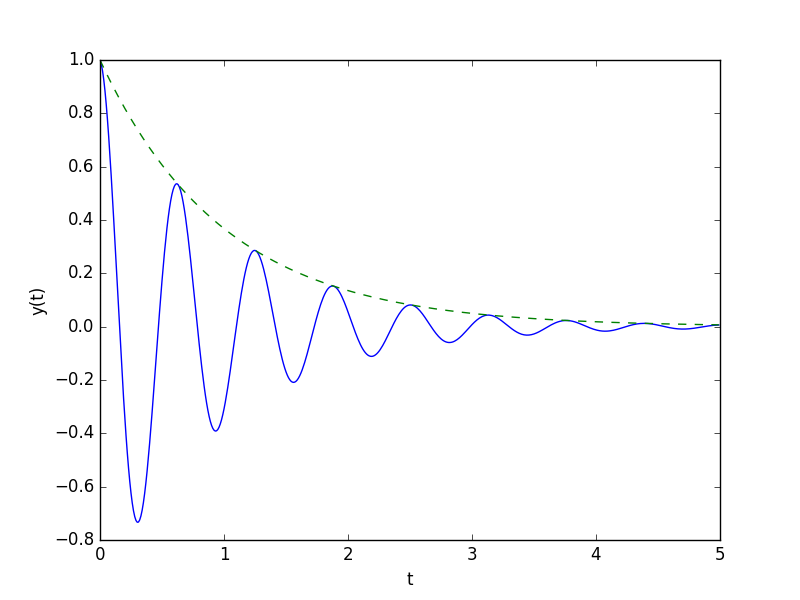
\includegraphics[scale=0.7]{Figures/under_damped.png}
    \caption{Under-Damped HO. The real part of the solution (blue), for the un-driven, under-damped harmonic oscillator.
    The dotted line (green) shows that the amplitude of the function (and the the function itself) slowly decays to zero over time.}
  \label{fig:under_damped}
\end{figure}
%=============================================================================80
%	            New Page To Make Figure Flow With Text                     %
%==============================================================================%
\newpage

\subsubsection*{Overdamping ($\omega_o < \gamma$)}
The overdamping case can be physically interpreted as having a very large friction contribution.
In the case of overdamping, the square root in equation \ref{eq:oscillator_char} is real not complex, so we can just write the general solution as
\be
\begin{split}
x(t) &= c_1 e^{-\gamma + \sqrt{\gamma^2 - \omega_o^2}} + c_2 e^{-\gamma - \sqrt{\gamma^2 - \omega_o^2}} \\
&= c_1 e^{-(\gamma - \sqrt{\gamma^2 - \omega_o^2})} + c_2 e^{-(\gamma + \sqrt{\gamma^2 - \omega_o^2})}
\end{split}
\ee
By rewriting the general solution we see what is happening to the oscillator's position, notice the two negative exponential terms.
In the case of overdamping, the resistive force, proportional to the damping constant, dominates the spring force.
So once the oscillator is kicked at time t $=$ 0, it will move to its maximum displacement and then quickly decay to zero displacement without anymore oscillations.

\subsubsection*{Critical Damping ($\omega_o = \gamma$)}
In the case of critical damping, the damping constant is equal to the natural frequency, $\lambda_+ = \lambda_-$.
To find the general solution, we must solve for repeated roots in the auxiliary equation.
The general solution can be written as
\be
x(t) = (c_1 + c_2t)e^{\lambda_+ t} = (c_1 + c_2t)e^{\lambda_- t}
\ee
With arbitrary constants $c_1$ and $c_2$.
This means that the characteristic equation has two equal roots
\be
\begin{split}
x(t) &= c_1 e^{\lambda_1 t} + c_2 te^{\lambda_2 t}\\
&= c_1 e^{-\gamma t} + c_2 te^{-\gamma t}\\
\end{split}
\ee
Here we see that our ODE is second order, and we get 2 free (potentially complex) parameters, meaning the dimensionality of the solution space is 2.

\subsection*{Inhomogeneous Linear ODE (constant Coefficients)}
The general form for an inhomogeneous equation with constant coefficients is given by
\be \label{eq:und_coeff_ex}
	\sum_{n=0}^N a_n x^{(n)} = f(t) .
\ee
A well known example (N=2) is the \textbf{Driven Harmonic Oscillator}.
Similar to the Damped Harmonic Oscillator, the differential equation for the Driven Harmonic Oscillator has the same LHS as the Damped non-driven case (see equation \ref{eq:damp_oscillator}) but the RHS has a function f(t) which is referred to as the driving force.

The general solution for any inhomogenous ODE is of the form
\be
x(t) = x_p(t) + \sum_{n=0}^N c_nx_n(t)
\ee
Where x$_p$(t) is a \textbf{Particular Solution} to the inhomogeneous equation, and x$_n$(t) = e$^{\lambda_n t}$.
This form can be used to solve any inhomogenous ODE by simply changing the value of N to fit the order of your ODE of interest.
Unfortunately there is no general method to solve for the particular solution.
But it is very convenient to use the \textbf{Method of Undetermined Coefficients} for this specific problem.
The following cases show you how to obtain the particular solution using this method (assuming that you have already solved for the homogenous solution).
As an example, we will consider different variations of the following ODE for each case to give you a better idea of how to apply the method.
\be
3 \frac{d^2 x}{dt^2} + x = f(t)
\ee

\subsubsection*{Case 1}
If we have f(t) = $Be^{\Omega t}$, we can assume the particular solution to be of the form $x_p(t) = Ae^{\Omega t}$.
Substituting this guess into the inhomogeneous equation gives us the value of A
\be
A \sum_{n=0}^N a_n \Omega^n e^{\Omega t} = B e^{\Omega t} \Rightarrow A = \dfrac{B e^{\Omega t}}{\sum\limits_{n=0}^N a_n \Omega_n e^{\Omega t}} \Rightarrow A = \dfrac{B}{\sum\limits_{n=0}^N a_n \Omega^n}
\ee
At no point did we assume $\Omega \in \Re$, so this derivation is in general complex. \bigskip

Now, let's consider a different ODE:
\be
3 \frac{d^2 x}{dt^2} + x = 4e^{\Omega t}
\ee
If we use our assumption $x_p(t) = Ae^{\Omega t}$, we can make the substitution
\be
3A\Omega^2e^{\Omega t} + Ae^{\Omega t} = 4e^{\Omega t} \Rightarrow 3A\Omega^2 + A = 4 \Rightarrow A = \frac{4}{3\Omega^2 + 1}
\ee
So our particular solution is
\be
x_p(t) = \frac{4}{3\Omega^2 + 1} e^{\Omega t}
\ee
Motivated readers are welcome to substitute in this solutiom to the ODE to confirm it is a solution.

\subsubsection*{Case 2}
Our next special case is of the form $f(t) = B_1e^{\Omega_1t} + B_2e^{\Omega_2t} + \hdots$
We can immediately guess a particular solution that is of the form $x_p(t) = A_1 e^{\Omega_1t} + A_2 e^{\Omega_2t} + \hdots$
Substituting this into the inhomogeneous equation (equation \ref{eq:und_coeff_ex}), we find (truncating to 2 terms for simplicity)
\be
A_1 e^{\Omega_1t} \sum_{n=0}^N a_n \Omega_1^n + A_2 e^{\Omega_2t} \sum_{n=0}^N a_n \Omega_2^n = B_1e^{\Omega_1 t} + B_2 e^{\Omega_2 t}
\ee
To make the math easier to handle, we can re-write this as a set of linear equations
\be
\begin{split}
   A_1 e^{\Omega_1 t} \sum_{n=0}^N a_n\Omega_1^n = B_1 e^{\Omega_1 t} \Rightarrow A_1 \sum_{n=0}^N a_n\Omega_1^n = B_1 \\
   A_2 e^{\Omega_2 t} \sum_{n=0}^N a_n\Omega_1^n = B_2 e^{\Omega_2 t} \Rightarrow A_2 \sum_{n=0}^N a_n\Omega_1^n = B_2
\end{split}
\ee
Once we have the solutions to both equations, we can combine them to form the particular solution for the total equation.
Since case 2 can be broken down into a set of linear equations that each resemble case 1, refer to the example in case 1 to see how the coefficients are determined.

\subsubsection*{Case 3}
What if our f(t) was of the form of a sine or cosine function?
In general, it is safer to assume that the particular solution is a linear combination of sine and cosine, and then let the math decide for itself which of the two (if not both) is truly necessary for the particular solution.
Notice, however, that we can also assume our solution to be a linear combination of exponential terms, by simply re-writing all sines and cosines using the following relationships.
\be
\begin{split}
    \cos(\Omega t) &= \frac{e^{i\Omega t} + e^{-i\Omega t}}{2}\\
    \sin(\Omega t) &= \frac{e^{i\Omega t} - e^{-i\Omega t}}{2i}\\
\end{split}
\ee
For example, let's consider the example ODE
\be
3 \frac{d^2 x}{dt^2} + x = 4\sin(t) .
\ee
We can assume that x$_p(t)$ = Acos(t) + Bsin(t) and make the necessary substitutions
\be
[-3A\cos{(t)} - 3B\sin{(t)}] + [A\cos{(t)} + B\sin{(t)}] = 4\sin{(t)} .
\ee
And after combining like-terms,
\be
- 2A\cos{(t)} - 2B\sin{(t)} = 4\sin{(t)}
\ee
We see that the only way for this equation to hold is by having $A = 0$ and $B = -2$. So our particular solution looks like
\be
x_p(t) = -2\sin{(t)}
\ee
If you haven't made the connection by now, you could have also assumed that the particular solution was just a function of sine and not cosine.
However, the reason why you could have done that in this example is because there are only even derivatives of the function x(t).
So if you only used sines, your derivatives would only give you sines and no cosines.
If the ODE had at least one odd derivative, a particular solution with only sines would not get you anywhere.
You can either take my word for it or try it for yourself by replacing the second derivative in this example with a first derivative, third derivative, etc, and substituting a guess that only contains a sine term.

\subsubsection*{Case 4}
Our next case assumes f(t) = $B_0 + B_1t + B_2t^2$. We can make the guess that $x_p(t) = A_0 + A_1t + A_2t^2$ and substitute it into equation \ref{eq:und_coeff_ex} (again, truncating to 2 terms for simplicity)
\be
a_0\left(A_0 + A_1t + A_2t^2\right) + a_1\left(A_1 + 2A_2t\right) + 2a_2A_2 = 0
\ee
This is a second order polynomial in t. Since we have 3 undetermined coefficients, we can create 3 equations to solve for each of them in order to obtain the particular solution.
\be
\begin{split}
    a_0A_0 + a_1A_1 + 2a_2A_2 &= B_0\\
    a_0A_1 + 2a_1A_2 &= B_1\\
    a_0A_2 &= B_2\\
\end{split}
\ee
Let's again consider an example ODE
\be
3 \frac{d^2 x}{dt^2} + x = (2-t)(t+2) .
\ee
Since $(2-t)(t+2) = 4 - t^2$, we can assume our guess is of the form $x_p(t)$ = $A_2t^2 + A_1t + A_0$.
Just as in case 3, we want to make sure our guess is general enough to describe the system.
We continue with the method by substituting into the original ODE
\be
3[2A_2] + [A_2t^2 + A_1t + A_0] = (2 - t)(t + 2) \Rightarrow A_2t^2 + A_1t + A_0 + 6A_2 = 4 - t^2
\ee
By inspection, we can see that since the RHS does not contain a coefficient multiplied by t, A$_1 = 0$.
So now we just need to make 2 equations to solve for the other 2 coefficients.
\be
\begin{split}
A_0 + 6A_2 &= 4\\
A_2 &= -1\\
\end{split}
\ee
So after determining coefficients, we can say that our particular solution is
\be
x_p(t) = -t^2 + 10
\ee

\subsubsection*{Case 5}
Our final case to consider is when f(t) = $(B_0 + B_1t + B_2t^2) e^{\Omega t}$.
By analogy to all the other cases, we can make our guess for the particular solution to be $x_p(t) = (A_0 + A_1 t + A_2 t^2) e^{\Omega t}$ and substitute into equation \ref{eq:und_coeff_ex}.
While this seems tedious to calculate, you will see that, despite having an exponential term, the problem can be reduced to case 4 because the exponential term can be cancelled out.
\be
\begin{split}
& a_0[ (A_0 + A_1 t + A_2 t^2) e^{\Omega t} ] + a_1[ (A_1 + 2 A_2 t) e^{\Omega t} + (A_0 + A_1 t + A_2 t^2) \Omega e^{\Omega t} ] + \\
& a_2[ (2 A_2) e^{\Omega t} + (2 A_1 + 4 A_2 t) \Omega e^{\Omega t} + (A_0 + A_1 t + A_2 t^2) \Omega e^{\Omega t}] \\
&= (B_0 + B_1t + B_2t^2) e^{\Omega t}
\end{split}
\ee
After dividing each term by $e^{\Omega t}$, you'll notice that it will look a lot like case 4, where will have a polynomial in t, but with $\Omega$ terms included.
\be
\begin{split}
& a_0[ (A_0 + A_1 t + A_2 t^2) ] + a_1[ (A_1 + 2 A_2 t) + (A_0 + A_1 t + A_2 t^2) \Omega ] + \\
& a_2[ (2 A_2) + (2 A_1 + 4 A_2 t) \Omega + (A_0 + A_1 t + A_2 t^2) \Omega] \\
&= B_0 + B_1t + B_2t^2
\end{split}
\ee
Then we just need to combine like-terms to get our coefficients, a$_0$, a$_1$, and a$_2$.
\be
\begin{split}
&(a_0 A_2 + a_1 A_2 \Omega + a_2 A_2 \Omega) t^2 + (a_0 A_1 + 2a_2 A_2 + a_1 A_1 \Omega + 4a_2 A_2 \Omega + a_2 A_1 \Omega) t \\
& + (a_0 A_0 + a_1 A_1 + a_0 A_0 \Omega + 2a_2 A_2 + 2a_2 A_1 \Omega + a_2 A_0 \Omega) \\
&= B_0 + B_1t + B_2t^2
\end{split}
\ee
\be
\begin{split}
    a_0(A_0 + A_0 \Omega) + a_1 A_1 + a_2(2 A_2 + 2 A_1 \Omega + A_0 \Omega) &= B_0 \\
    a_0 A_1 + a_1 A_1 \Omega + a_2(2 A_2 + 4 A_2 \Omega + A_1 \Omega) &= B_1 \\
    a_0 A_2 + a_1 A_2 \Omega + a_2 A_2 \Omega &= B_2 \\
\end{split}
\ee
Remember that A$_1$, A$_2$, and A$_3$ are known values, so we end up with our system of 3 linear equations to solve for our 3 unknowns.

And this is the last special case that Vladimir knows how to solve analytically!

The Method of Undetermined Coefficients is a simple method to help solve inhomogenous equations with constant coefficients.
It only requires you to make your guess for the particular solution mimicing the form of f(t), and it's just algebra from there!

\subsection*{Linear ODE with Variable Coefficients}
Constant coefficient linear ODEs can be solved with linear algebra as we saw.
Unfortunately, problems with variable coefficients are a bit more tricky.
There is not a general approach to solve these problems and it is often done numerically rather than analytically.
We can try to use methods mentioned before such as the Variation of Parameters or Method of Undetermined Coefficients but it is not guaranteed to always work.
There are even other methods that are usually covered in undergraduate differential equations courses, but we will not go over them here.

A famous example of a second order variable coefficient ordinary differential equation is the 1-D Schr\"odinger Equation!
\be
-\frac{\hbar^2}{2m} \Psi''(x) + [E - V(x)] \Psi(x) = 0
\ee
Here, V(x) is changing (it is a function of x), which means that the coefficient of the ODE changes in x along with the function $\Psi$.
The SE is a good example to use because the equation is always used in Quantum Mechanics. In most Quantum Mechanics courses, we discuss different scenarios where the potential V(x) takes on different forms.

If our potential takes the form of the potential for a Harmonic Oscillator (V(x) = kx$^2$) we can get analytic solutions to this differential equation.
Some other examples of linear ODEs with variable coefficients are the Morse Potential, and a piecewise constant potential.

\begin{figure}[H]
    \centering
    \begin{subfigure}[b]{0.49\textwidth}
        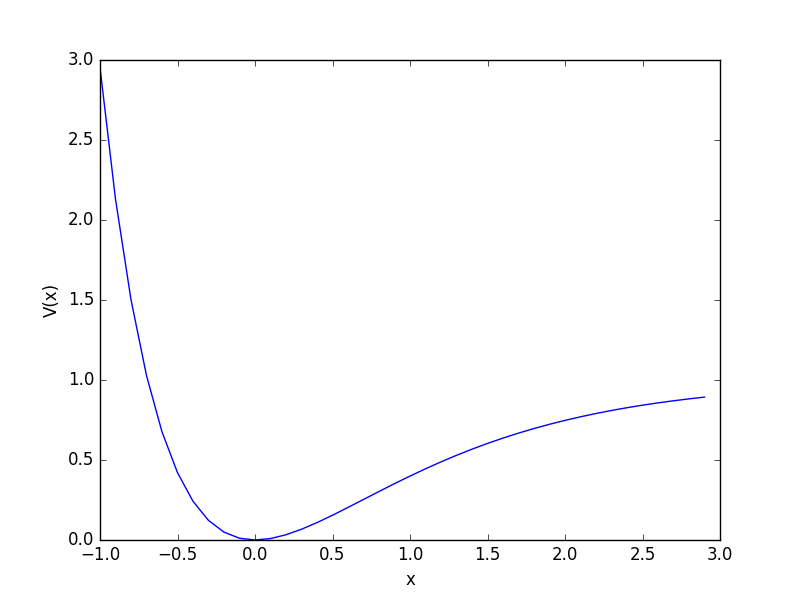
\includegraphics[width=\textwidth]{Figures/morse.png}
  	\caption{The Morse Potential.}
    \end{subfigure}
    \begin{subfigure}[b]{0.49\textwidth}
        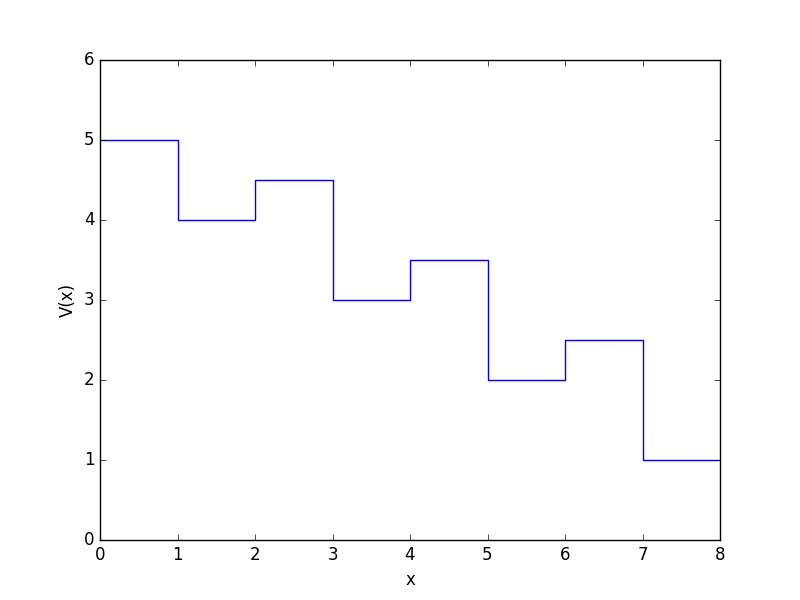
\includegraphics[width=\textwidth]{Figures/piecewise.png}
        \caption{The Piecewise Potential.}
    \end{subfigure}
    \caption{Potentials for Linear ODEs with Variable Coefficients}
\end{figure}

Another example of a second order, variable coefficient ODE is the Vertically/Horizontally Forced Pendulum.
As the name implies, this system consists of having a pendulum attached to an object that is moving vertically and/or horizontally.
Obtaining the equation of motion for the system is non-trivial and is often done using Lagrangian mechanics instead of Newtonian mechanics.
Since this is not a physics course, we will not derive the equation and only show you that the equation can be approximated as
\be
u'' + (\alpha + \beta\cos(t)) u = 0 .
\ee
You can see that one of the coefficients in the equation depends on t, this makes the equation a second order, linear, homogenous, non-constant coefficient ODE.

This problem is very interesting, if you allow the focal point where the pendulum connects to the base to move you can generate a stable solution to the problem.
All of these examples are just to motivate the problems, we do not need to know these specific cases.

\end{document}
